\documentclass[conference]{IEEEtran}
\IEEEoverridecommandlockouts
% The preceding line is only needed to identify funding in the first footnote. If that is unneeded, please comment it out.
\usepackage{cite}
\usepackage{amsmath,amssymb,amsfonts}
\usepackage{algorithmic}
\usepackage{graphicx}
\usepackage{textcomp}
\usepackage{xcolor}
\usepackage{booktabs}
\usepackage{float}
\usepackage[hidelinks]{hyperref}
\usepackage{minted}
\usepackage{biblatex} %Imports biblatex package
\addbibresource{ref.bib} %Import the bibliography file

\def\BibTeX{{\rm B\kern-.05em{\sc i\kern-.025em b}\kern-.08em
    T\kern-.1667em\lower.7ex\hbox{E}\kern-.125emX}}

\begin{document}

\title{Solving Lunar lander problem with multiple uncertainties and continuous action
space using Deep Deterministic Policy Gradient\\

{\footnotesize Report - ACIT4630 2024 - Group 5}\\
\vspace{-15}
{\footnotesize Oslo Metropolitan University (OsloMet)}\\
\vspace{-15}
{\footnotesize Oslo, Norway}
 
}
 
\author{
  \begin{tabular}[t]{@{}l@{}}
    \normalsize Mehdi Heidari \\
    \normalsize s338859@oslomet.no \\
    \small ACIT Master Student
  \end{tabular}
  \and
  \begin{tabular}[t]{@{}l@{}}
    \normalsize Mahendran Sharujan Karthigesu \\
    \normalsize makar8270@oslomet.no \\
    \small ACIT Master Student
  \end{tabular}
  \and
  \begin{tabular}[t]{@{}l@{}}
    \normalsize Terje Saltskår \\
    \normalsize s351881@oslomet.no \\
    \small ACIT Master Student
  \end{tabular}
}
\maketitle

\begin{abstract}
This study presents a reinforcement learning approach to address the complexities of the Lunar Lander problem in a continuous action space with multiple uncertainties such as variable gravity and wind conditions. By integrating the Deep Deterministic Policy Gradient (DDPG) framework with enhancements such as recurrent neural network layers and a refined experience replay mechanism, we develop a robust system capable of adapting to non-Markovian environments. Our model shows in managing dynamic uncertainties, making significant strides towards more intelligent and adaptable autonomous spacecraft control systems. This research underscores the potential of advanced reinforcement learning techniques in improving the precision and safety of spacecraft landings in unpredictable conditions. The implementation details and source code for this project are available at: https://github.com/TerjeOtsal/4630-LunarLander-
\end{abstract}

\begin{IEEEkeywords}
Luner Lander, OpenAI Gym, DDPG, PyTorch, Uncertainties, Continuous Control, Reinforcement Learning, Q-learning, Critic Network.
\end{IEEEkeywords}


\section{Introduction}
Introduction Space discovery and, therefore, the successful
sending and landing of an aircraft on various space bodies have
problems that require existing and control procedures, which
are both intelligent and resilient. The open-source agent is
intended to solve the lunar lander mission, a two-dimensional
simulation created by OpenAI, and thus to land safely and
efficiently on a moon-like surface by the spacecraft. The earlier
works have shown their efficiency in solving this problem
without uncertainties. However, real-life phenomena are full
of stochastic behaviors, such as variable starting positions,
gravity, and wind, and they form a more complex scenario
for the further development and improvement of reinforcement
learning algorithms. As against Q-learning, modern reinforce-
ment learning algorithms use Markovian environments in
which it is assumed that future states depend only on the
current state and action. Though this assumption may closely
approximate the reality in scenarios and simulations with no
uncertainties, it is impractical in the actual environment as the
past actions decide the states, and the current state governs the
future \cite{parsons2015virtual}.

Conventional RL algorithms face a problem in dealing with non-Markovian phenomena because they are incapable of capturing all the necessary information needed for truly solving the underlying issue that the non-Markovian phenomenon brings, necessitating the development of more sophisticated approaches. However, in this case, a Deep Q-Learning (DQL) approach has become a solution that is highly likely to succeed. By using the ability of the neural networks and feeding in the information about the experiences of past state-action pairs \cite{candadai2020sources}. In addition to multilevel planning, it ensures the withstanding of uncertainties and serves as a strong base for problem-handling in deep action spaces.
 
\section{The Lunar Lander Environment}

The Lunar Lander environment, a popular benchmark in reinforcement learning, simulates the task of autonomously landing a spacecraft on the surface of the moon. Developed as part of the OpenAI Gym toolkit, this environment provides a rich and challenging domain for testing and developing reinforcement learning algorithms. The objective is straightforward yet complex: navigate the lander to touchdown at a designated landing pad, marked by a flag. However, accomplishing this feat involves managing a continuous action space and optimizing a reward system that mimics the balance required for a soft landing. The simulation incorporates various physical forces, including gravitational pull and environmental resistance, making the task dynamic and the outcome uncertain. Success in this environment demands precise control, foresight, and adaptability, reflecting real-world challenges faced in actual lunar landing missions \cite{palanisamy2018hands}.

\subsection{Continuous action space}
In contrast to environments with discrete action spaces, The Lunar Lander can also operate within a continuous action space. This allows for much more nuanced controls that are more realistic compared to environments in real-life tasks. The difference between the discrete action spaces 4 possible actions : fire main thruster, left oriented thruster, right oriented thruster and doing nothing, is that in a continuous action space the thrusters can be adjusted between 0 and 1 leaving a close to infinite possible combinations of actions. Applications like the Lunar Lander are especially well suited for algorithms like the Deep Deterministic Policy Gradient (DDPG), which excels in handling continuous action spaces \cite{Gjersvik2019LandingMoon}

\subsection{Rewards and Penalties}

The reward system in the Lunar Lander environment is designed to encourage behaviors that nudge the agent towards better solutions that lead to a successful and safe landing. Most of the Rewards work similarly to the discrete action space where the possible rewards and penalties are as follows: The Lunar Lander will gain points based on its position compared to the position of the goal. it will also gain a reward based on its velocity while landing to ensure that the agent attempts to slow the descent down to a safe speed. Furthermore the agent will also gain a penalty or reward based on the angular momentum while landing. It also gains 10 points for each of its legs that land and 100 points for a safe landing.Where the continuous action space rewards differ from the discrete ones at the thruster rewards. The max throttle for the main thruster is ten times stronger in the discrete action space and the penalty for using the engines are therefore 0.3 points per frame for the main thruster and 0.03 points for the side thrusters. In the continuous action space on the other hand the penalty per second is based on how hard the agent decides to run the engines.



\section{Background/Related Work}


\subsection{Reinforcement Learning in Discrete and Continuous Action Spaces}
Reinforcement learning has been divided into two predominant approaches: discrete and continuous action spaces.\cite{han2019energy} Conventional DQL strategies that utilize techniques like Q-learning have been extensively used in the cases of action spaces with the presence of distinguished actions, as every action can be assessed individually. Conversely, in continuous action spaces, the approach must be defined to generate multiple actions at a time, not just having a predefined set of actions. While this problem is still standing, some recently created strategies, like Deep Deterministic Policy Gradient (DDPG) and Proximal Policy Optimization (PPO), are attempting to make models that can output a broad spectrum of actions \cite{guttulsrud2023solving}. Thus, these techniques have made reinforcement learning possible in tasks requiring exact control, such as in robotics and autonomous systems. The DDPG and PPO methods permit agents to learn state-to-action policies that directly map states to continuous actions\cite{tang2020discretizing}, making these methods more refined and flexible, increasing their performance in tasks with actions that are not discrete but instead are along a continuous.


\subsection{Handling Uncertainties in Reinforcement Learning}
The adjustment of the networks to deal with uncertainties associated with an environment that varies its features, such as gravity or wind resistance, thus providing a non-Markovian aspect of reinforcement learning tasks. Such a situation deviates from the classical framework, in which, most importantly, actions taken and states experienced during the past have their impact on the current state, but only through the current state. Keneshloo et al. (2019)\cite{keneshloo2019deep} proved this by using DQL-STM, which allowed the agent to incorporate past state-action pairs, predicting better changes and quickly reacting to the environment dynamics. Therefore, through applications of short-term memory techniques, DQL-STM agents can manage the non-Markovian orderliness by paying attention to both the contents and the ordering of the observations in a sequence as well as can help it in better decision-making \cite{guttulsrud2023solving}. This combination of prior encounters leads the agents to gather experience and make necessary changes to the employed strategies that help them be more successful in complex and unpredictable environments.


\subsection{Challenges in Continuous Control}
In this adaptation, all action spaces transition from discrete to continuous control. The current framework implements modifications of the reward mechanisms, including the state representations, to provide more precise control. For instance, an on-off type reactionary Lunar Lander model would not be able to learn any difference in the engine coke due to the difference in the intensity thrust over the course of a running continuous process\cite{elkins2020adaptive}. It would know multiple accelerations as well as the correlated factors of the actions of landing.

Primarily, the facet of continuous actions is that they prepare these learning curves for a broader scope of possible actions on their way forward. Approaches such as DDPG and PPO have become solutions to these challenges. This is because agents can, therefore, learn policies that, without restriction, can directly transform the current state of the environment into the desired action. The implication is that those same agents now have a bigger play space to play with, allowing them to carry out finer modifications or more precise controls during the landing maneuvers\cite{dulac2021challenges}. Through this upgrade, both the controls have become more realistic, accurate, and swift than in real situations.

\subsection{Contribution from related work}
A recurrent neural network layer inside the architecture of the DDPG agent, captures the temporal dependencies by receiving the current state and a sequence of past state-action pairs as input. It can contribute to a historically informed political and critical organizational network, improving decision-making processes. Furthermore, our models use methods like experience replay to interrupt temporal correlations and target networks for better stability and convergence\cite{li2017deep}. The proposed design aims to achieve this goal with an integrated solution, which would work as a robust and adaptive control framework for Lunar Lander using deep reinforcement learning techniques and historical context.

\subsection{Proposed Solution}
To solve the Lunar Lander problem with several variables of uncertainty in the continuous space, we propose a novel methodology that merges the DDPG algorithms \cite{arxivContinuousControl}. Our solution integrates the DQL approach developed by Håkon Guttulsrud\cite{guttulsrud2023solving}. Our system consists of a DDPG agent. Where DDPG has proved itself to be a mighty algorithm for solving continuous control problems by becoming an amalgam of Q-learning and policy gradient approaches. As a result, the agent is empowered to output continuous actions directly.

Nevertheless, DDPG has a problem handling non-Markovian environments in which early actions and states profoundly influence future states that the Q-function incorporates as an essential element. To deal with this drawback, we suggest our innovation of upgrading the DDPG agent. A particular case of this module, which keeps track of such a buffer of state-action pairs in the past, is helping the agent to use this historical background during its activity. In such a way, real-time information can be maintained, and the variables of the environment can be measured, including the effects of uncertainties such as variable gravitation and wind conditions\cite{hazrathosseini2024transition}.

The module, part of the DDPG agent's nervous system and implemented as a recurrent neural network layer, perceives all past state-action pairs as the current state and extracts temporal dependencies since it receives the current state and a sequence of past state-action pairs as input. This is a way of taking control of the context, helping it capture and control the actor and critic networks better, thereby influencing decision-making, usually based on historical factors. Besides the methods of experience replaying, for example, to destroy temporal correlations, we might also take the networks for the targets to achieve more excellent stability and convergence. Such integration leads to our solution that can provide an effective and adaptive source of control for the Lunar Lander problem – the problem of continuous action spaces under uncertainties – with the help of deep reinforcement learning and factors inherent in historical time.

\subsection{Discussion}

The suggested solution opens amid many Lunar Lander problems with a persistently faulty action space and complex physics. Our approach is based on the DDPG architecture to enable the agent to tackle the non-Markovian environment and learn policies relying on previous experience. The DDPG framework is one of the bases because it allows the agent to see the present state dynamically and to track the patterns and allegories that reveal the future state. Past historical states must be considered because they control future dynamics. Consequently, the DDPG approach, which has shown a positive influence on continuous control of such complex manoeuvres in landing on the Moon, is used with the view of precise control of the spacecraft's movement necessary for a smooth landing\cite{guttulsrud2023solving}. 
Implementing within the DDPG architecture is a keypoint in the framework we utilize. The transition buffer is efficiently updated with state transitions, and the use of recurrent neural network layers allows our agent to learn how these transition patterns in the past were connected to other subsequent state´s evolutions\cite{goudarzi2021distributed}. The contextualization of historical acts is critical in uncertain surroundings involving the variation of gravity and wind speeds because past performance of operations and existing states greatly influence future dynamics of the system.

Additionally, our proposal demonstrates the benefits of DDPG in the continuous control domain, thus helping the agent to produce policies that send the exact continuous actions. This ability is the core requirement for the Lunar Lander problem, where the strength and direction of the spacecraft's jets must be monitored carefully to ensure a successful landing\cite{hossny2021refined}. We generalize our DDPG method with the mechanisms to take into account not only the non-Markovian properties of the environment but also provide us with the means of making the spacecraft's movements more fine-grained.

In addition to the primary technology, our solution incorporates several machines and deep reinforcement learning approaches to enhance the agent's learning and adaptation capabilities. Experience replay is a memory that not only performs a replay of previous actions but also learns the action from the memory buffer. This allows agents to learn more effectively. Moreover, experience replay solves the cyclic issues. Similar to existing methods, our approach is advantageous in its combination, particularly in employing reinforcement learning tailored for precise control operators in continuous tasks, especially within challenging conditions\cite{liu2018effects}. Incorporating non-Markovian features of the environment and control at the finest level spearheads the creation of more advanced agents that can operate through different situations and use vast numbers of robotic, autonomous systems or the like. 

However, these concerns do exist and challenge my proposed solution. Execution of this method, along with its appraisal, is a resource-consuming and challenging task that is often accomplished through the help of super-strong computers and a proper estimate of the hyperparameter tuning. Besides that, we are evaluating the methods developed above on various scenarios like other domains and different weather conditions by pursuing more experiments.

\section{Uncertainties}
To create a more realistic simulation we used three of the built-in uncertainties from the Lunar-Lander v2 environment. This accompanied by a continuous action space led to more realistic and challenging simulations to land in. The uncertainties we introduce for this paper are gravitational pull, Turbulence and Wind speed. These uncertainties make the environment too hard to navigate given only the current state and thus making it non-Markovian.

\subsection{Gravitational Pull}
To simulate landing on different celestial bodies, we introduce variable gravitational forces between -12 to 0. This variation forces the agent to calibrate the use of the thruster dynamically, requiring it to adjust its strategy depending on the force as on planets with stronger gravitational force, more fuel must be used to stabilize the lander. Whereas a weaker gravitational force might lead to overcompensation and instability.

\begin{figure}[htp]
    \centering
    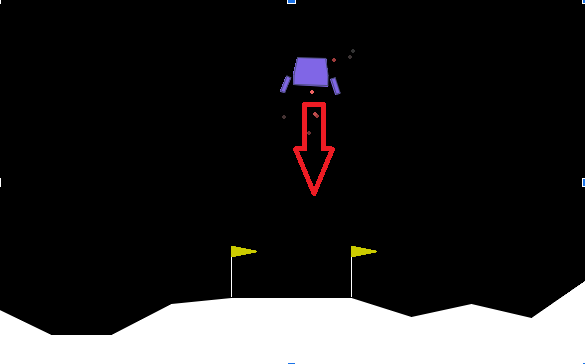
\includegraphics[width=0.3\textwidth]{images/image 1.png}
    \caption{Illustrating Gravitational Pull}
    \label{Illustrating Gravitational Pull}
\end{figure}
%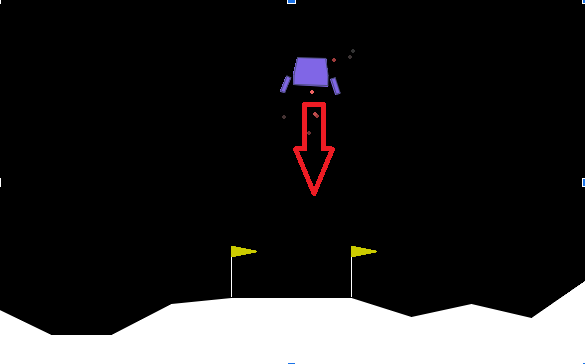
\includegraphics[width=5cm, height=4cm]{images/image 1.png}

\subsection{Turbulence}
In real life scenarios, atmospheric turbulence can significantly affect both the descent and landing of a spacecraft, similarly to how airplanes deal with turbulence during landing and take off. We introduced turbulence as random variations in wind speed and direction affecting the lander as it descends. Turbulence affects the stability of the lander, testing the agent’s ability to maintain control in unpredictable conditions.

\begin{figure}[htp]
    \centering
    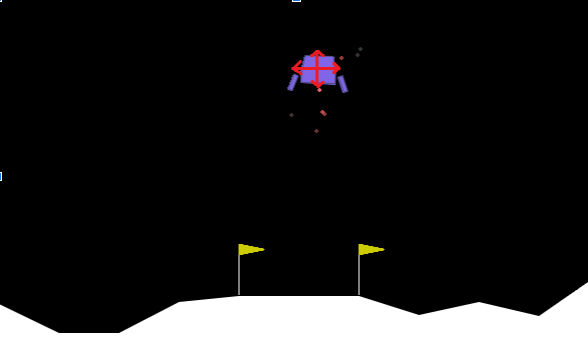
\includegraphics[width=0.3\textwidth]{images/image 2.PNG}
    \caption{Illustrating Turbulence}
    \label{fIllustrating Turbulence}
\end{figure}


\subsection{Wind}
In our Lunar Lander environment, wind is introduced to apply another layer of complexity and realism. In our environment the wind speed can vary between 0 and 20 units, and its direction is randomized across 360 degrees. The unpredictability of the wind requires the agent to continuously adjust its navigation strategy, promoting a much more robust and versatile agent. The wind’s impact highlights the importance of real time decision making in the agent's architecture. See fig \ref{fig:Illustrating Wind}

\begin{figure}[htp]
    \centering
    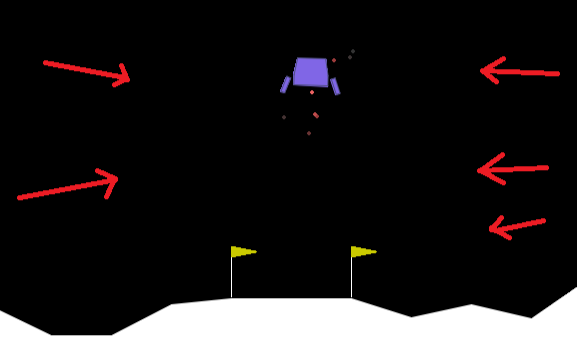
\includegraphics[width=0.3\textwidth]{images/image 3.PNG}
    \caption{Illustrating Wind}
    \label{fig:Illustrating Wind}
\end{figure}



\section{Model Architecture and Dynamics}
We introduce an advanced reinforcement learning framework employing a Continuous Actor-Critic architecture enhanced with sophisticated action noise integration to tackle complex, dynamic simulations such as the Lunar Lander. This model is built upon the deep deterministic policy gradient (DDPG) approach, refined by incorporating real-time environmental variability, thereby enhancing its adaptability to unpredictable scenarios\cite{zhong2019deep}.

\subsection{Network Structure}
The network structure consist of two principal components designed for efficiency and robust response for many variable conditions:

\subsubsection{Actor Network}
Responsible for determining the most suitable action for the current state, the Actor Network functions by:
\begin{itemize}
    \item Input Layer: Takes in the complete state representation from the environment
    \item Hidden Layers: Consist of two layers “fc1\_dims” and “fc2\_dims” with 600 and 450 units respectively, these layers are equipped with layer normalization and the ReLU activation function to enhance the network’s ability to learn patterns more efficiently.
    \item Output Layer: Utilizes a hyperbolic tangent function to ensure that the action values are within the expected bounds for the environment's continuous action space.
\end{itemize}
    
\subsubsection{Critic Network}
Evaluates the potential of the actions taken by the Actor by estimating their Q-values through a similar structure to the Actor Network\cite{sung2017learning}.
\begin{itemize}
    \item Input Layer: Integrates the state and action values to assess the complete state-action scenario.
    \item Hidden Layers: These layers have structural likeness to the ones in the Actor Network, however here the action values are introduced into the second layer to directly predict the actions potential rewards.
    \item Output Layer: Outputs a scalar Q-value indicating the predicted reward efficacy of the state-action pair.
\end{itemize}

\subsection{Enhancements and Optimizations}
\subsubsection{Ornstein-Uhlenbeck Action Noise}
To facilitate enhanced exploration, especially in environments with continuous action spaces, our model integrates Ornstein-Uhlenbeck (OU) action noise. This type of noise, which introduces temporally correlated variations to the actions, aids in overcoming the limitations of standard uncorrelated noises by encouraging more strategic exploration patterns. This exploration strategy is pivotal in navigating environments that require precise control and is in line with findings from recent research demonstrating the benefits of such noise types over conventional methods in deep reinforcement learning \cite{eberhard2022pink}.

\subsubsection{Replay buffer Mechanism}
The Replay Buffer is an essential tool in our model for mitigating the correlation among sequential actions and thereby stabilizing learning updates. As identified by Di Castro et al. (2022) \cite{di2022analysis}, the stochastic processes within a Replay Buffer can de-correlate data samples effectively, enhancing the learning process by providing a randomized sample of experiences. This functionality is crucial in our framework, enabling the agent to learn from a diverse set of experiences, thus preventing overfitting and improving the generalization of the learned policies.

\subsubsection{Training procedure}
The Learning algorithm utilizes the Adam optimizer for efficient backpropagation error minimization, with separate learning rates for the Actor (0.0002) and Critic Network (0.002), optimizing the convergence rate.
To stabilize the effects of rapidly changing policy updates, soft target updates are employed. This method gradually blends in the weight of the target network with the main networks, ensuring that new experiences don’t have a drastic impact and keeps the policy evolution stable.

\section{Experiment}
Our experiments focused on evaluating the performance of the Deep Deterministic Policy Gradient (DDPG) model under a series of environmental conditions that include variable wind, turbulence, and different gravitational pulls. These conditions are specifically designed to test the robustness and adaptability of the DDPG agent in handling more dynamic and unpredictable scenarios that closely mimic real-world situations.

\subsection{Experimental Setup}
Each experimental run was designed to test the impact of the individual hyperparameters such as the learning rates (‘alfa’ and ‘beta’), Batch sizes, and Network dimensions. These parameters were then systematically tweaked to better isolate their effects. The model was implemented using Python and PyTorch framework. As the goal of the testing was to optimize the hyperparameter set, batch sizes and values were adjusted as testing proceeded.

\subsubsection{Uncertainty Modeling}
The environmental uncertainties, wind, turbulence and gravitational variations were all introduced from the beginning of each experiment to better gauge how our proposed model managed to overcome the difficulties from scratch. For wind and turbulence, the intensity and direction were randomized within predefined ranges to simulate changing atmospheric conditions. For gravity, values were adjusted to simulate different planetary conditions, ranging from moon-like to Earth-like gravity.
The wind is randomly adjusted within a range of 0 to 20 m/s, the Turbulence is varying between mild to more severe levels and is parameterized with a scaling factor between 0,5 and 2.0 and the gravitational force is set between a downwards force of -12 to 0. 

\subsection{Testing methodology}

To better gauge the impact of the different parameters, we designed our testing protocol that allowed us to observe the impact on the learning trajectory of a new untrained agent. Applying all the uncertainties from the beginning of each experiment meant that the agent had to learn in as realistic of an environment as is possible and lead to the agent getting rewards and penalties that are realistic to the environment it is meant to solve. 
While testing, a window rendering how the model is actually working in the Lunar Lander environment is always open to allow testers for easier understanding of its current strategy. This is important as it lets us visually see what is hindering the agent from achieving better results as well as showing how the agent is handling the continuous action space.

\subsubsection{Hypermeter Evaluation}
The primary focus of each test was to evaluate how different hyperparameter settings influenced the ability of a completely untrained agent to learn and perform effectively in the Lunar Lander environment. Specifically, we aimed to determine if the agent could converge to an average score of approximately 200 points, indicative of successful landings, or if it would plateau at lower scores, signaling less optimal performance. Each hyperparameter was adjusted individually across successive tests to isolate its effects and to edge the Model towards better and more efficient training \cite{guttulsrud2023solving}.

\begin{figure}[htp]
    \centering
    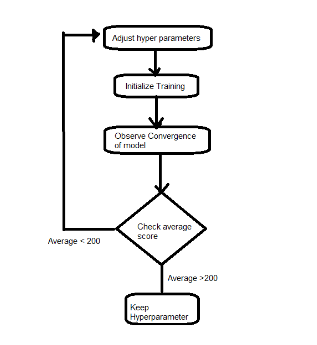
\includegraphics[width=0.4\textwidth]{images/image 4.PNG}
    \caption{Flowchart illustrating the Hyperparameter testing to evaluate the best set for training the Agents}
    \label{fig:Flowchart for hyperparameter testing}
\end{figure}
%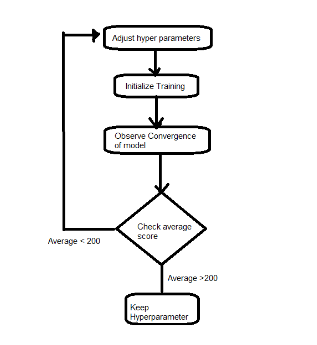
\includegraphics[width=5cm, height=4cm]{images/image 4.PNG}

\section{Results}
To provide a comprehensive view of the agent’s learning process, the average of the previous 100 scores was plotted (figure 5), the graph shows a clear upwards trend, that indicates that the agent learned and improved its performance throughout the episodes. The agent’s performance eventually stabilized and consistently hit the 200-point threshold, which is considered a successful and safe landing in the ‘LunarLander-v2’ environment. 

This Agent then demonstrated robust performance across 50 evaluation episodes. The scores per episode are depicted in Figure 6, and the agent scores around 220 to 320 points per episode. The variability in the scores between 220 to 320 points suggests that while the agent performs well overall, there are occasional deviations which could be due to stochastic elements within the environment. This highlights the importance of continued exploration and adaptation during training to handle unexpected scenarios effectively.

The agent's ability to not only reach 200 points but stabilize and consistently land safely demonstrates its proficiency in handling the ‘LunarLander-v2’ environment. The stability in the running average plot further confirms that the training process effectively enhanced the agent’s capabilities. The agent’s success can be attributed to the design of the network architecture and the use of techniques such as the Ornstein-Uhlenbeck noise process to encourage the agent to explore when faced with sub-optimal solutions. This can be derived through the dips in Figure 5 as the agents were able to adapt and overcome by exploring new possible solutions.
\begin{figure}[htp]
    \centering
    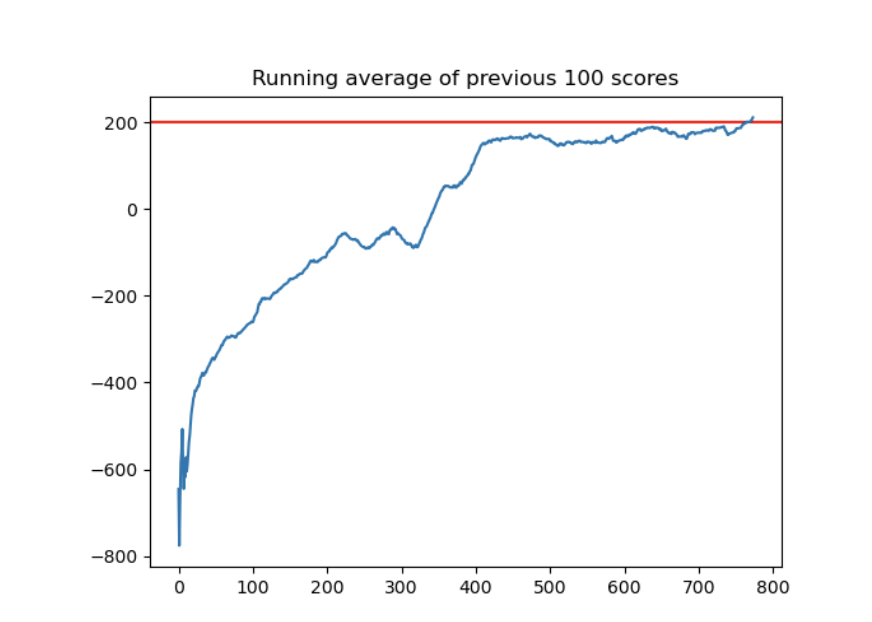
\includegraphics[width=0.4\textwidth]{images/image6.png}
    \caption{Running average of previous 100scores}
    \label{fig:Average Score}
\end{figure}

\begin{figure}[htp]
    \centering
    \includegraphics[width=0.4\textwidth]{images/image8.PNG}
    \caption{Performance of Trained Model}
    \label{fig:Trained Model}
\end{figure}


\section{Discussion}
The results demonstrate the agent's substantial learning and adaptation capabilities within the 'LunarLander-v2' for continuous action space environment. The consistent achievement of high scores, coupled with the observed stability in performance, highlight the effectiveness of the DDPG approach and the network architecture. The integration of Ornstein-Uhlenbeck noise facilitated exploration, enabling the agent to overcome sub-optimal solutions and adapt to varying scenarios highlights the importance of exploration strategies in reinforcement learning. Furthermore, the observed variability in scores suggests that the agent can handle unexpected events, indicating a robust and flexible learning process. Future research could explore more advanced noise processes or adaptive exploration techniques to further enhance performance.

\section{Conclusion}
In conclusion, our proposed system is a step towards overcoming the difficulties of multiple uncertainties within continuous action space in the problem of Lunar Lander. This approach integrates Deep Deterministic Policy Gradient (DDPG) by imposing the Actor Network, which, along with supplementary stabilization techniques, strives to promote an efficient and flexible control mechanism that can manage intelligently in a complex environment. Incorporating advanced reinforcement learning technologies helps thoroughly  dynamical behavior, allowing the spacecraft to act and adapt to any situation in real time while ensuring their safety and efficiency. The refinement and experimentation of our approach could bring along improvements in autonomous spacecraft control systems' capacity and, therefore, contribute to future exploration and exploitation of space.

\section{Future Work}
While the agent performed really well with the uncertainties provided within the ‘LunarLander-v2’ environment, there are several areas for future research.
\begin{itemize}
\item Complex environment: testing the agent in more challenging environments with uncertainties as randomized starting position, could provide extra insights into its adaptability and robustness.

\item Alternative Algorithms: Comparing the current approach with alternative reinforcement learning algorithms, such as Twin Delayed DDPG (TD3), could help identify potential performance gains \cite{openaiTwinDelayed}.

\end{itemize}


\printbibliography %Prints bibliography

\onecolumn
\section{Appendix}
\subsection{Contribution}

This project was a collaborative effort, with each participant contributing 100\%. The specific contributions are as follows:
\begin{itemize}
\item Mahendran Sharujan Karthigesu
makar8270@oslomet.no:  Conducted extensive research and gathered previously known versions of the code, aswell as refining the code we provided.

\item Terje Saltskar
s351881@oslomet.no: Made significant contributions to testing parameters, code structure, and the code for running the finished agent.

\item Mehdi Heidari
s338859@oslomet.no: Focused on developing and refining the code architecture, ensuring the model's effective implementation for the project. 
\end{itemize}

\subsection{Code Appendix}

\begin{itemize}
\item This project aim to solve The Lunar Lander environment for a continious action space using a DDPG algorithm.

\item Nothing except for the necessary imports are needed to run the DDPG implementation script.

\item The finished model is in the actor.pth and is called into the trainedmodel.py file for demonstration. 

\item To run the provided script, you need to have the following packages installed:
\begin{minted}[fontsize=\tiny]{python}
numpy (version 1.21.0)
torch (version 1.9.0)
gym (version 0.21.0)
matplotlib (version 3.4.2)
You can install these packages using the following pip commands:
pip install numpy==1.21.0
pip install torch==1.9.0
pip install gym==0.21.0
pip install matplotlib==3.4.2
\end{minted}

\item LunarLander-v2 Agent: This project implements a Deep Deterministic Policy Gradient (DDPG) agent to solve the LunarLander-v2 environment from OpenAI Gym.

\item Installation: To set up the environment, install the following dependencies:

\begin{minted}[fontsize=\tiny]{python}
```bash
pip install numpy==1.21.0
pip install torch==1.9.0
pip install gym==0.21.0
pip install matplotlib==3.4.2

python trainedmodel.py

\end{minted}

\item To run the dppg\_implementation.py use python dppg\_implemeentation.py. Keep in mind this will reset the weights of the current actor.pth file!



\end{itemize}
\end{document}